\newpage
\section{Proof of Proposition \ref{thm:improvement}}
\label{app:proof}
\begin{proof}
\textbf{Baseline.}  
In sequential execution, each of the $T$ steps requires one call to the true model $h$ with mean latency $1/\beta$. Therefore
\[
E[T_{\mathrm{seq}}] \;=\; \frac{T}{\beta}.
\]

\medskip
\textbf{Expected time saved per hit.}  
Consider two consecutive steps $(t,t{+}1)$. In the baseline, the total completion time is $R = B + C$, where $B,C \sim \mathrm{Exp}(\beta)$ are the latencies of step $t$ and step $t{+}1$. With speculation, we launch $A \sim \mathrm{Exp}(\alpha)$ during step $t$. If the guess is correct, the $(t{+}1)$ call $C$ can be issued once either $A$ or $B$ finishes, so the block completes at
\[
S \;=\; C + \min\{A,B\}.
\]

Thus, when a guess is correct, our expected time saved is
\[
R - S \;=\; (B-A)_+,
\]
where $(x)_+ = \max\{x,0\}$.
  
By independence of $A,B$,
\[
\mathbb{E}[(B-A)_+]
= \int_{0}^{\infty}\!\int_{0}^{b} (b-a)\,\alpha e^{-\alpha a}\,\beta e^{-\beta b}\,da\,db
= \frac{\alpha}{\beta(\alpha+\beta)}.
\]

\medskip
\textbf{Expected number of hits}. We denote the expected number of hits by round $n$ as $S_n$, that is
$$\E[\text{number of hits by round }n] = S_n$$
We then have $S_0=0$, $S_1 = p$. In round $1$, either (i) we hit with probability $p$, in which case round $2$ cannot be a hit (there is no speculation window immediately after a correct speculation), contributing $1+S_{n-2}$; or (ii) we miss with probability $1-p$, after which round $2$ proceeds normally, contributing $S_{n-1}$. We then have the following recursion
$$S_n = p(1+S_{n-2}) + (1-p)S_{n-1}$$
Solve this linear recurrence by splitting into homogeneous and particular parts.

\textit{(1) Homogeneous part}
\[S_n^{h} = pS_{n-2}+ (1-p)S_{n-1}\]
The characteristic equation is
\[
r^2-(1-p)r-p=0=(r-1)(r+p) \implies \text{the roots are }r_1=1, r_2=-p
\]
Therefore,
\[
S_n^{(h)}=C_1 + C_2(-p)^n.
\]

\textit{(2) Particular solution}
The forcing term is constant ($+p$), and $r=1$ is a root, so a constant trial collides with the homogeneous part. Try $S_n^{(p)}=an$ and substitute:
\[
an=(1-p)a(n-1)+pa(n-2)+p
= an - a(1+p) + p,
\]
which gives $a(1+p)=p$ and thus
\[
S_n^{(p)}=\frac{p}{1+p}\,n.
\]

Combine:
\[
S_n = C_1 + C_2(-p)^n + \frac{p}{1+p}\,n.
\]
Use $S_0=0$ and $S_1=p$:
\[
0=C_1+C_2,\qquad
p=C_1 + C_2(-p) + \frac{p}{1+p}.
\]
Solving yields $C_2=-\dfrac{p^2}{(1+p)^2}$ and $C_1=\dfrac{p^2}{(1+p)^2}$.

Hence the closed form solution is
\[
S_n=\frac{p}{1+p}\,n+\frac{p^2}{(1+p)^2}\Bigl(1-(-p)^n\Bigr)
\]

\medskip
\textbf{Total saving.}  
There are $T-1$ potential speculation windows, hence
\[
E[T_{\mathrm{s}}]
= \frac{T}{\beta} - S_{T-1}\frac{\alpha}{\beta(\alpha+\beta)}
\]

\medskip
\textbf{Final ratio.}  
Dividing by $E[T_{\mathrm{seq}}] = T/\beta$ gives
\[
    \frac{E[T_{\mathrm{s}}]}{E[T_{\mathrm{seq}}]}
    \;=\;
    1 - \frac{1}{T}\frac{\alpha}{\alpha+\beta}\left[\frac{(T-1)p}{1+p}+\frac{p^2}{(1+p)^2} - \frac{p^2}{(1+p)^2}(-p)^{T-1}\right]
\]
\end{proof}
Taking $T\to\infty$, we get exactly that the ratio converges to $1-\frac{p}{1+p}\frac{\alpha}{\alpha+\beta}$




\section{Additional Environment Details}
\label{app:additional_details}

\subsection{Chess}
\begin{figure}
    \centering
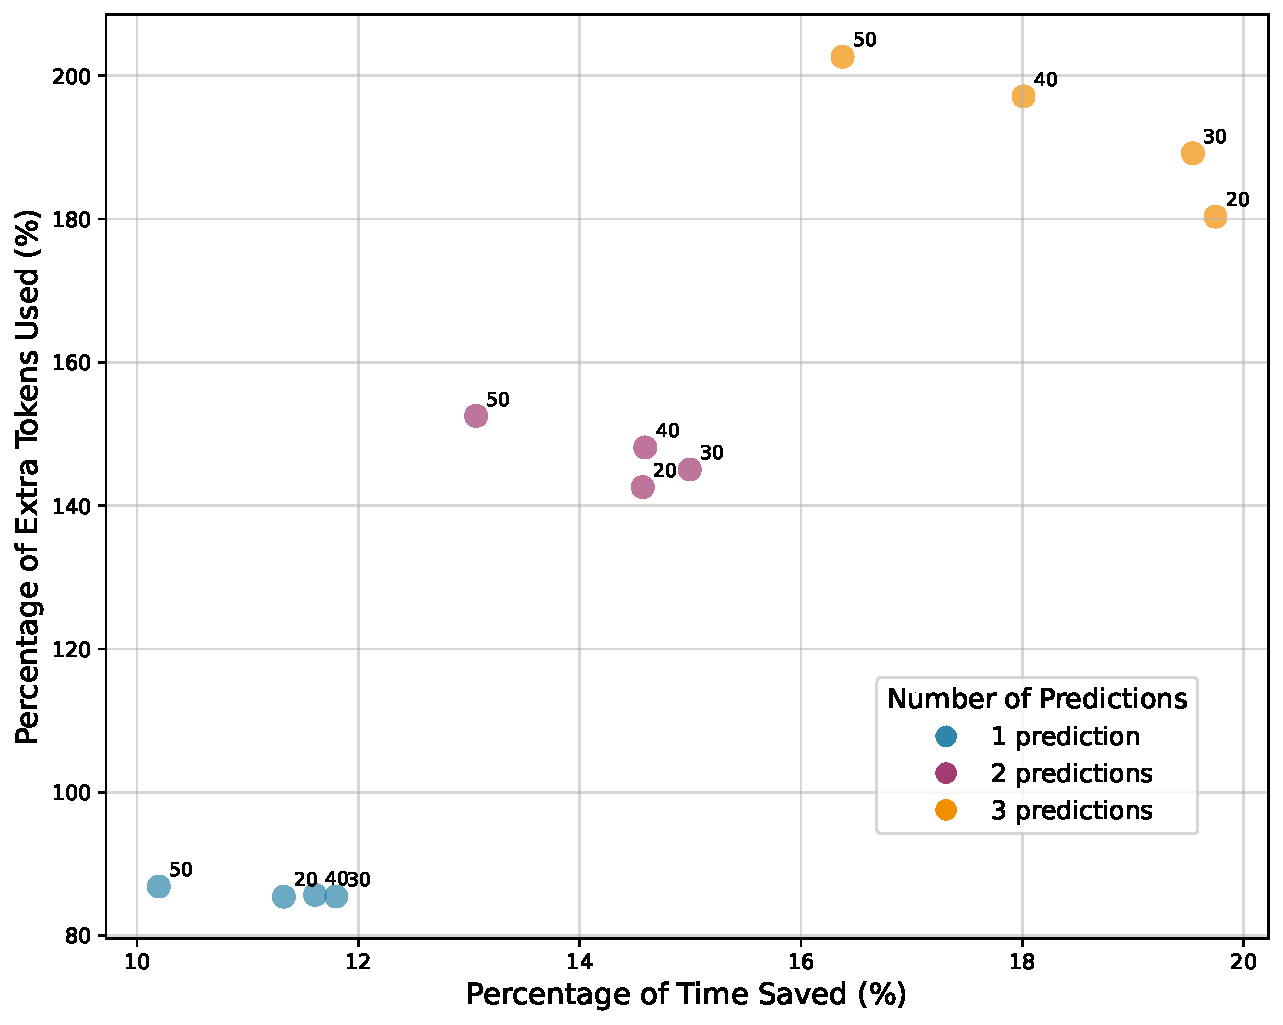
\includegraphics[width=0.6\linewidth]{figures/chess/combined_time_token_plot.pdf}
    \caption{Percentage of extra tokens used against percentage of time saved for different numbers of predictions at different numbers of steps, averaged across $5$ runs.}
 \label{fig:chess_time_token_plot}
\end{figure}

\paragraph{Trade-off between Time Saved and Token Cost.} In addition to time savings, we also measure the additional token cost of parallel speculation. We track this using the metric \textbf{extra token percentage}: $(M_{sequantial}-M_{speculative})/{M_{sequential}}$. Figure~\ref{fig:chess_time_token_plot} shows the trade-off between time saved and token cost for each number of predictions. We observe that the extra token percentage increases as the number of predictions increases, while the time saved percentage also increases, creating a clear trade-off.

\subsection{Ecommerce}
% \begin{wrapfigure}{r}{0.45\columnwidth}
%     \centering
%     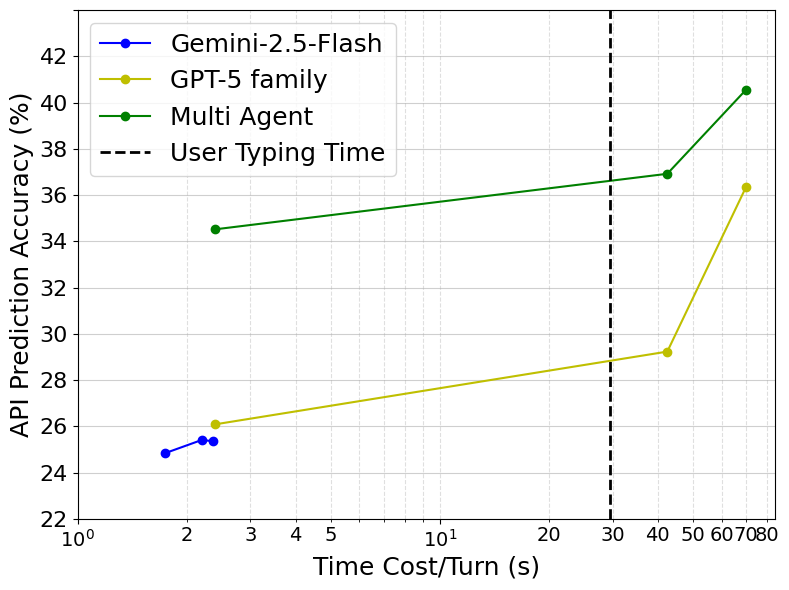
\includegraphics[width=\linewidth]{figures/ecommerce/time_accuracy.png}
%     \caption{Prediction accuracy versus speculation time. Blue and yellow curves show single-agent speculation, while the green curve shows the multi-agent setting. The dashed vertical line indicates average user typing time.}
%     \label{fig:time_accuracy}
% \end{wrapfigure}

\paragraph{$\tau$-bench:} A benchmark designed for dynamic task-oriented dialogues between a user (simulated by language models) and an API-augmented agent. The benchmark spans two domains — retail and airline, with structured databases, domain-specific tools. We focus on the retail domain, where the agent assists users with operations such as canceling or modifying pending orders, initiating returns or exchanges, or providing product and order information. The benchmark defines 115 tasks with 15 APIs (7 write, 8 read-only).

\paragraph{Trade-off between Prediction Accuracy and Cost.}
The time cost in Figure~\ref{fig:time_acc} consists of latency (Time to First Token) and output response time. The dashed vertical line represents the average user typing time, estimated at 40 words per minute. At this threshold, the multi-agent setting achieves approximately 34\% prediction accuracy, meaning that in over one-third of cases the agent can return an immediate response without waiting for API execution. This demonstrates that speculation can transform user experience from perceptibly laggy to effectively real-time in tool-heavy environments.

\begin{figure}[H]
  \centering
  \resizebox{0.8\textwidth}{!}{%
      \begin{subfigure}[t]{0.48\textwidth}
        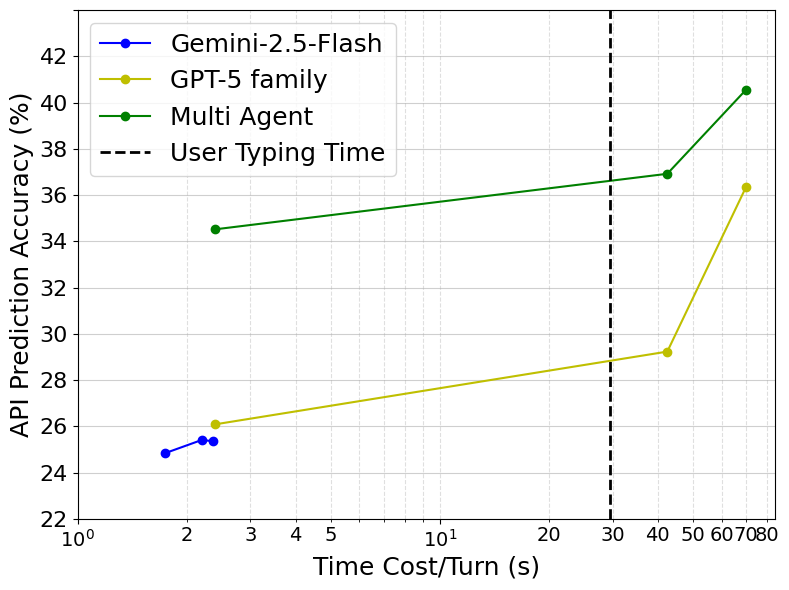
\includegraphics[width=\linewidth]{figures/ecommerce/time_accuracy.png}
        \caption{}
        \label{fig:time_acc}
      \end{subfigure}
      \hspace{0.05\textwidth} 
      \begin{subfigure}[t]{0.48\textwidth}
        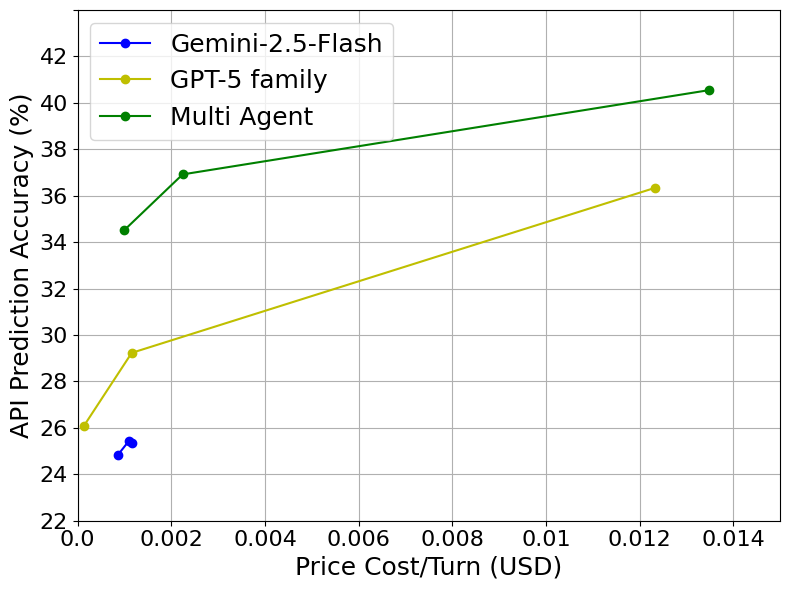
\includegraphics[width=\linewidth]{figures/ecommerce/price_accuracy.png}
        \caption{}
        \label{fig:price_acc}
      \end{subfigure}
  }
  \caption{\textbf{Prediction Accuracy against Speculator's Cost across different models.} (a) Accuracy–Speculator time cost trade-off across models. The dashed line shows average user typing time. (d) Accuracy–Speculator price trade-off across models, reflecting the monetary cost of speculative execution.}
  \vspace{-1em}
\end{figure}

\subsection{Operating System Tuning}
\newcommand{\ttt}[1]{\texttt{#1}}

\subsubsection{Experimental Setup and Implementation Details}

\paragraph{System and Workload Configuration}
All experiments were conducted on a dedicated machine with 2$\times$ Intel Xeon Silver 4114 10-core CPUs at 2.20 GHz, 192 GB DDR4 RAM, and a 1 TB NVMe SSD running Ubuntu 22.04 with Linux Kernel 5.15, hosted on Cloudlab~\citep{Duplyakin:ATC19}.

We run \ttt{sysbench cpu}~\citep{sysbench}, a CPU-bound benchmark that repeatedly calculates a large prime number sequence. The benchmark reports several performance metrics every second. We run sysbench on 16 concurrent threads pinned on two CPU cores.
\paragraph{Tuner Implementation Details}
The system consists of two agents, a fast Speculator and a slow Actor, which collaborate to minimize the p95 latency of the workload. At each step, the tuner proposes a new configuration, which is applied to the live system. Applying the proposed parameters is a near-instant operation.

\paragraph{CFS Parameter Details}
The Completely Fair Scheduler (CFS) is a CPU scheduler for Linux that aims to give every task a fair share of CPU time. It exposes various hyperparameters that allow administrators to adjust its behavior. We tuned \ttt{min\_granularity\_ns}, which enforces a minimum timeslice a task will receive. The prompt templates guided the agents to explore a range from 50,000 to 50,000,000 nanoseconds (0.05 ms to 50 ms). The default value on Kernel 5.15 is 3 ms. Lower values for this parameter are expected to increase responsiveness at the cost of higher context-switching overhead, while higher values improve throughput but can worsen latency.

\paragraph{History Compression}
\label{app:history_os}
History compression is managed via distinct prompt structures for the two agents. When the slower Actor is invoked, its prompt context contains a fully compressed summary of all actions taken during its deliberation window. Each action from the Speculator is listed as a concise (parameter, result) pair. In contrast, the faster Speculator receives a hybrid context: it sees the same compressed history from the last Actor cycle, supplemented by the full, verbose replies from its own most recent actions. This dual-context mechanism allows the Actor to analyze long-term trends from a compact summary, while the Speculator retains immediate, detailed context for its rapid, reactive decisions.


\subsubsection{Prompt Engineering for Multi-Agent Optimization}
\label{app:prompt_os}
The following are the prompt templates used to guide the two LLM agents.

\begin{tcolorbox}[
  enhanced,
  colback=gray!5!white,
  colframe=gray!60!black,
  title=Initial System Prompt for Actor and Speculator,
]
\small{
You are a Linux kernel scheduler tuning expert with deep knowledge of the Completely Fair Scheduler (CFS).\\

MULTI-AGENT ROLE: You are part of a MULTI-AGENT System.


[\textbf{For Actor}]
You are the Actor. Your role is to provide thoughtful, well-analyzed parameter recommendations. You work alongside a Speculator that explores the parameter space rapidly. You will receive accumulated results from multiple agent calls to perform deeper analysis and identify trends.\\

[\textbf{For Speculator}]
You are the Speculator. Your role is to provide immediate, intuitive parameter recommendations for each window. You work alongside an Actor that performs deeper analysis.\\

Your goal is to MINIMIZE p95 latency for a CPU-bound workload. The workload performance metrics might be NOISY, so look for consistent trends across configurations.\\

Tunable CFS parameter:
\begin{itemize}
    \item \ttt{min\_granularity\_ns}: Minimum time slice before preemption. Lower values increase responsiveness but also overhead. Higher values improve throughput but can worsen latency.
\end{itemize}

Parameter Range:
\begin{itemize}
    \item \ttt{min\_granularity\_ns}: 50,000 to 50,000,000 nanoseconds
\end{itemize}

Performance data will be provided in future calls. Respond ONLY in the format shown below:\\

\ttt{Analysis: <Your one or two-sentence decision reasoning>}\\
\ttt{Config: \{ "min\_granularity\_ns": <int> \}}
}
\end{tcolorbox}



\begin{tcolorbox}[
  breakable,
  enhanced,
  colback=gray!5!white,
  colframe=gray!60!black,
  title=Update for Speculator,
]
\small{

[\textit{Context includes the compressed history for calls 1-10 and the raw Speculator responses for iterations 11-18}]\\

CURRENT BEST: p95 latency=[value] at call \#[value]\\

Latest Result for call \#19: \\
Config: {"min\_granularity\_ns": [value]} $\rightarrow$ p95 latency=[value]\\

Please provide your analysis and the next configuration for iteration \#20.
}
\end{tcolorbox}

\begin{tcolorbox}[
  breakable,
  enhanced,
  colback=gray!5!white,
  colframe=gray!60!black,
  title=Update for Actor,
]

\small{

[\textit{Context includes the compressed history for calls 1-10}]\\

CURRENT BEST: p95 latency=[value] at call \#[value]\\

RESULT for call \#11 [SPECULATOR]: min\_granularity\_ns=[value] $\rightarrow$ p95 latency=[value]\\
RESULT for call \#12 [SPECULATOR]: min\_granularity\_ns=[value] $\rightarrow$ p95 latency=[value]\\
~...\\
RESULT for call \#19 [SPECULATOR]: min\_granularity\_ns=[value] $\rightarrow$ p95 latency=[value]\\

Please provide your analysis of the trend and the next configuration for call \#20.\\
}
\end{tcolorbox}


\begin{tcolorbox}[
  breakable,
  enhanced,
  colback=gray!5!white,
  colframe=gray!60!black,
  title=Sample Agent Response,
]
\small{
Analysis: The performance peaked at 300,000 ns, suggesting the optimal value is likely in that region. I will narrow the search around that peak.\\
Config: \{ ``min\_granularity\_ns'': 250000 \}
}
\end{tcolorbox}

\subsubsection{Token Usage and Costs}

\begin{figure*}[h]
  \centering
  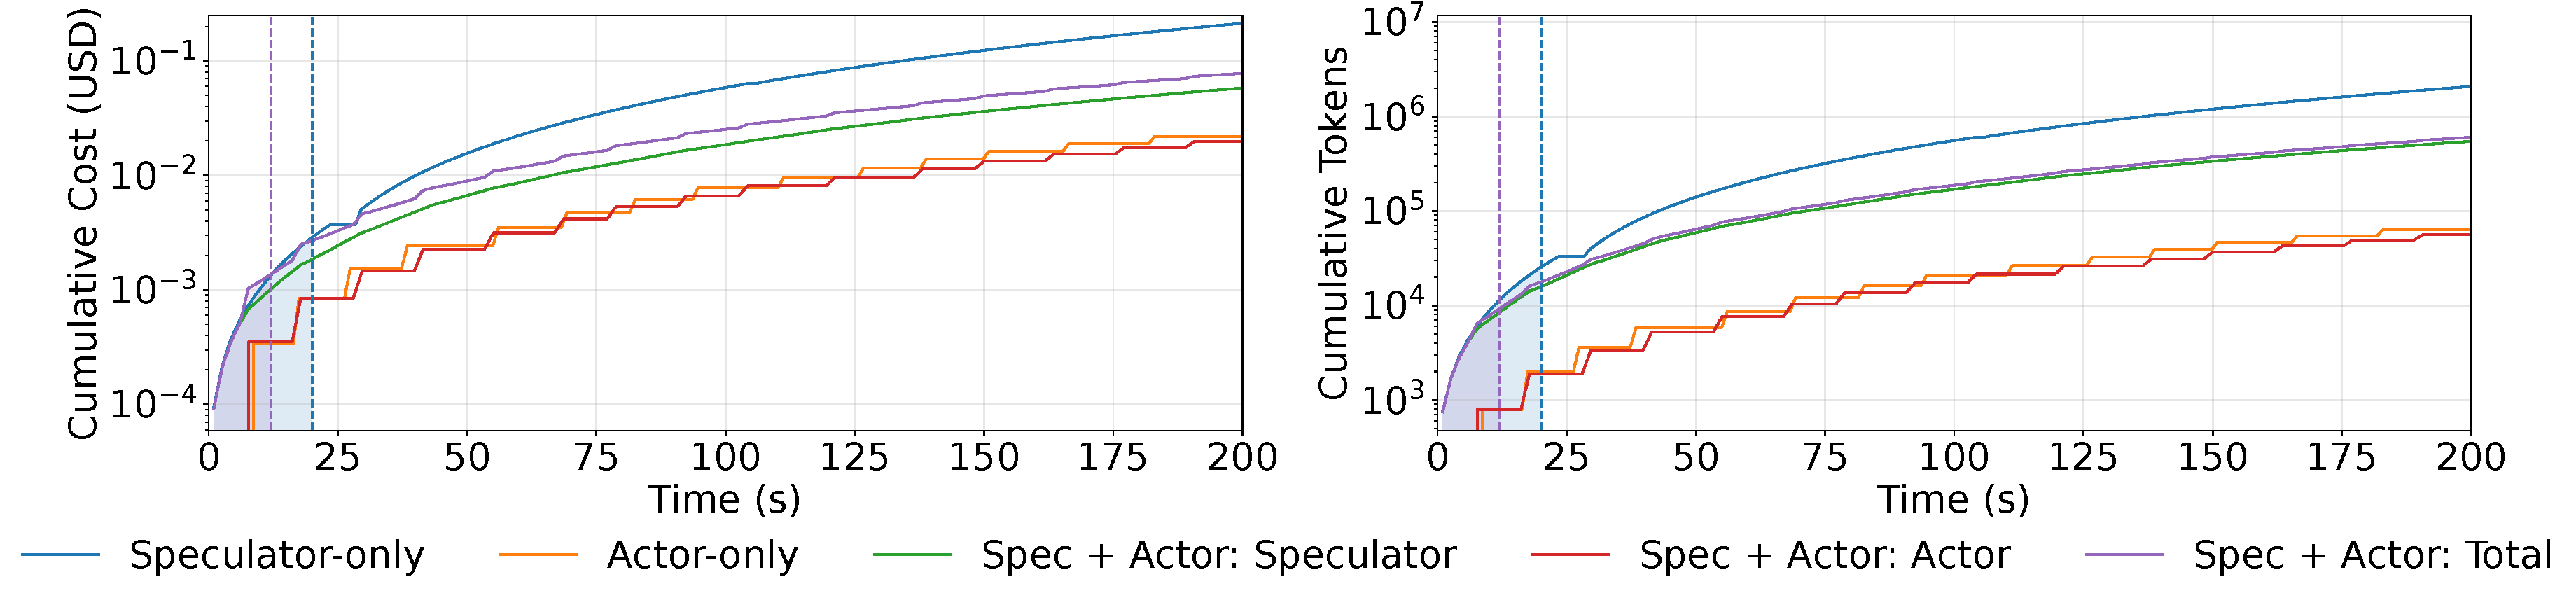
\includegraphics[width=\linewidth]{figures/os_tuning/cost.pdf}
  \caption{\textbf{Cumulative token usage and cost over time.}
  The left and right plots show the cumulative cost (USD) and total tokens used, respectively, for all three configurations.
  The vertical lines mark the observed convergence point for each system.}
  \label{fig:costs}
\end{figure*}


\begin{table*}[ht]
\centering
\caption{Cumulative tokens and cost (in cents) at selected time marks.}
\label{tab:costs}
\begin{tabular}{lrrrrrr}
\toprule
& \multicolumn{2}{c}{Actor-only} & \multicolumn{2}{c}{Speculator-only} & \multicolumn{2}{c}{Actor+Speculator (Total)} \\
\cmidrule(lr){2-3}\cmidrule(lr){4-5}\cmidrule(lr){6-7}
\textbf{Elapsed Time} & \textbf{Tokens} & \textbf{Cost (cents)} & \textbf{Tokens} & \textbf{Cost (cents)} & \textbf{Tokens} & \textbf{Cost (cents)} \\
\midrule
Base   & 744   & 0.02 & 690 & 0.01 & 690 & 0.03 \\
10s & 790   & 0.03 & 9,539 & 0.11 & 8,548   & 0.13 \\
30s & 3,631   & 0.15 & 45,768 & 0.57 & 32,459 & 0.48 \\
60s & 8,581   & 0.35 & 205,794  & 2.24 & 84,568 & 1.18 \\
120s  & 26,398 & 0.96 & 778,253  & 8.12 & 261,855  & 3.53 \\
200s & 63,376 & 2.18 & 2,099,894 & 21.5 & 607,877 & 7.83 \\
\bottomrule
\end{tabular}
\end{table*}

As illustrated in Figure~\ref{fig:costs} and detailed in Table~\ref{tab:costs}, the high frequency of the Speculator leads to rapid growth in token consumption and cost. In practice, however, this growth is bounded by the system's fast convergence. The combined Actor-Speculator system converges in approximately 15 seconds, while the Speculator-only system converges in 20 seconds. The Actor-only system converges after 200 seconds. Once an optimal state is reached, the tuning process concludes, rendering the potential for long-term exponential cost negligible in this context. Several optimization strategies, like truncating the context to a fixed window or disabling exploration after convergence, could further mitigate token growth but are left for future work.

\subsubsection{Speculative Reaction Time Benefits}
\label{app:speculative-mitigation}

To provide a targeted example of how speculation mitigates transient performance loss, we conducted a controlled experiment. In this scenario, the system is deliberately perturbed at time $t_0$ by setting the \ttt{min\_granularity} parameter to a highly suboptimal value (10 ms). We then compare the system's recovery under two configurations: the Actor-Speculator system and an Actor-Only baseline, which replays only the actions proposed by the Actor from the full Actor-Speculator trace.

\begin{figure}[h!]
  \centering
  
\includegraphics[width=0.6\linewidth]{figures/os_tuning/comparison.pdf}
  \caption{A controlled experiment showing the system's step response after a manual perturbation at $t=0$. The \textbf{Actor-Speculator} system corrects the poor setting within a second, while the \textbf{Actor-only} system must wait over 10 seconds for its next decision cycle. The quantitative results of this experiment are summarized in Figure~\ref{fig:os-speculation} (Right) in the main text.}
  \label{fig:os-reaction-appendix}
\end{figure}

As shown in Figure~\ref{fig:os-reaction-appendix}, the Actor-Speculator system reacts almost instantly. The fast Speculator, seeing the immediate performance degradation, applies a corrective action that brings the system back to an efficient state in about one second. In contrast, the Actor-Only system is forced to endure the poor performance for over 10 seconds, as it must wait for the slower Actor to complete its deliberation cycle before it can act.
The performance gap shown in the plot is quantified in the main text (Figure~\ref{fig:os-speculation}, Right).
